\section{Resultados}

Nesta seção, serão apresentados os resultados dos métodos numéricos aplicados à
função \textbf{\(\boldsymbol{\sin(x) + \cos(x) + 1}\)} com uma tolerância de
\textbf{0,000001}.

\subsection{\textbf{Resultados Gerados Por Cada Método}}

\subsubsection{\textbf{Método da Bisseção}}

Através da utilização do método da bisseção, partindo dos valores iniciais
$[1.1, 3.9]$, chegamos à raiz 3,141592, gerando o seguinte gráfico:

\begin{figure}[H]
	\centering
	\setlength{\fboxsep}{0pt}
	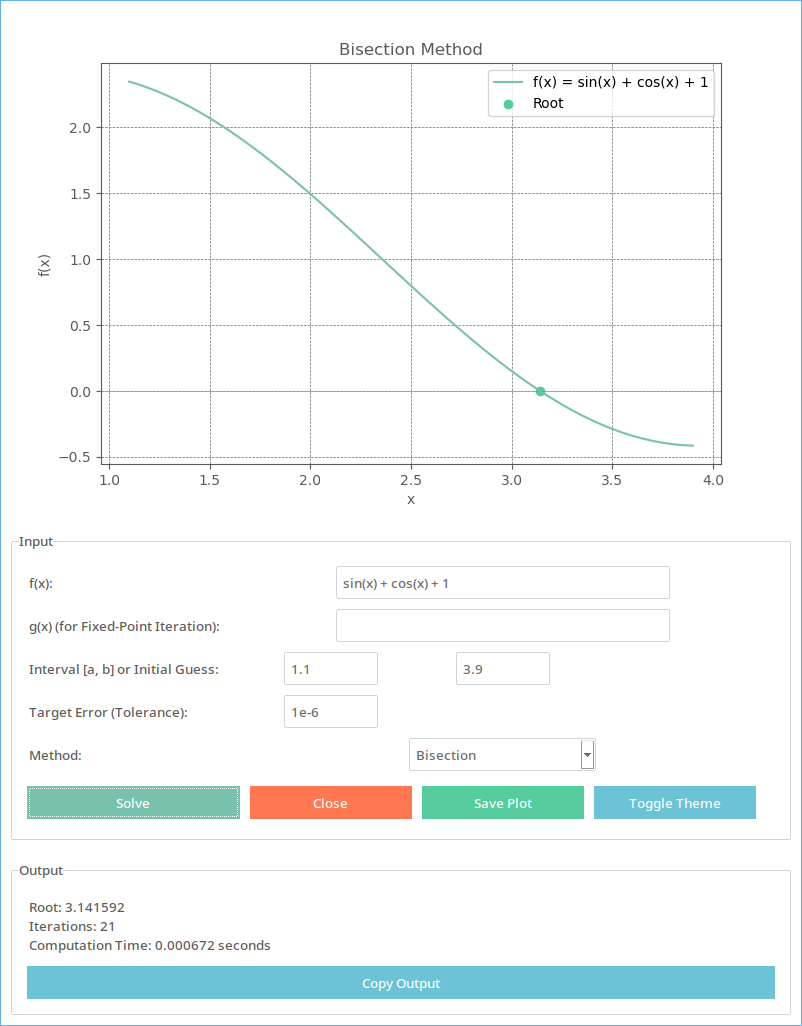
\includegraphics[height=0.5\textwidth]{./fig/bissecao.png}
	\caption{Gráfico da bisseção $[1.1, 3.9]$.}
	\label{fig:grafico-da-bissecao}
\end{figure}

\subsubsection{\textbf{Método de Newton-Raphson}}

Utilizando o método de Newton-Raphson com uma estimativa inicial de $[1.1,
			3.9]$, encontramos a raiz 3,141593 em 8 iterações. O gráfico abaixo ilustra a
convergência do método:

\begin{figure}[H]
	\centering
	\setlength{\fboxsep}{0pt}
	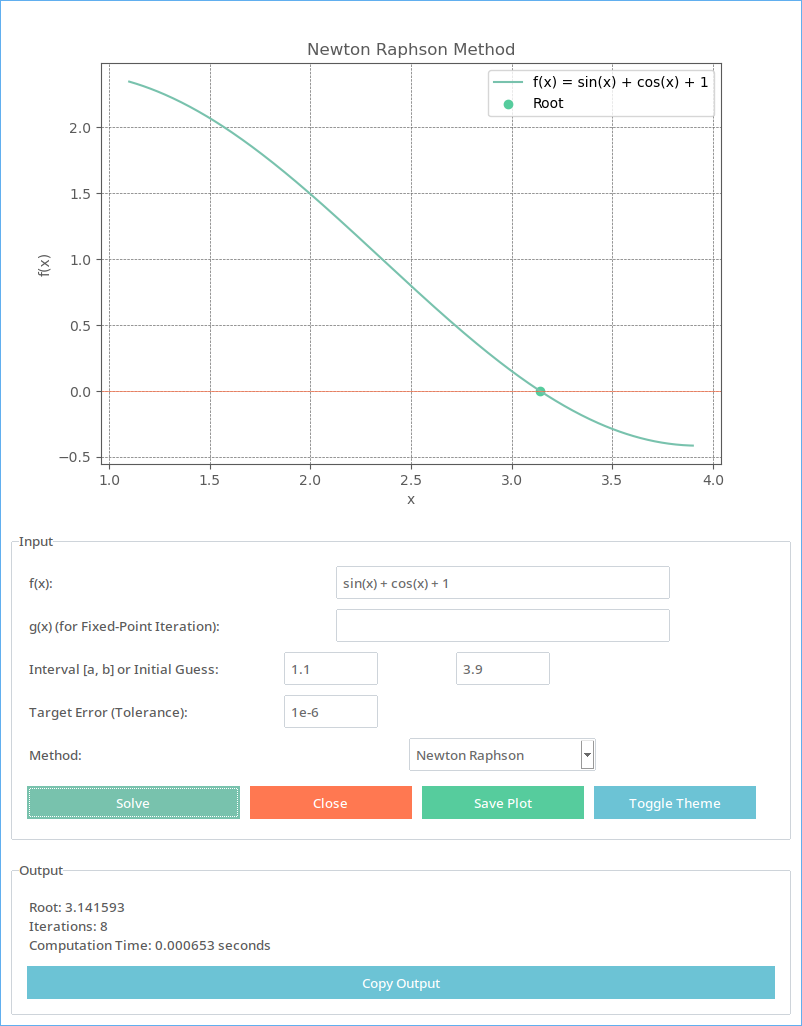
\includegraphics[height=0.5\textwidth]{./fig/newton-raphson.png}
	\caption{Gráfico newton-raphson $[1.1, 3.9]$.}
	\label{fig:grafico-newton-raphson}
\end{figure}

\subsubsection{\textbf{Método da Falsa Posição}}

Com o método da falsa posição, partindo do intervalo $[1.1, 3.9]$, obtivemos a
raiz 3,141593 em 7 iterações. O gráfico a seguir mostra o comportamento do
método:

\begin{figure}[H]
	\centering
	\setlength{\fboxsep}{0pt}
	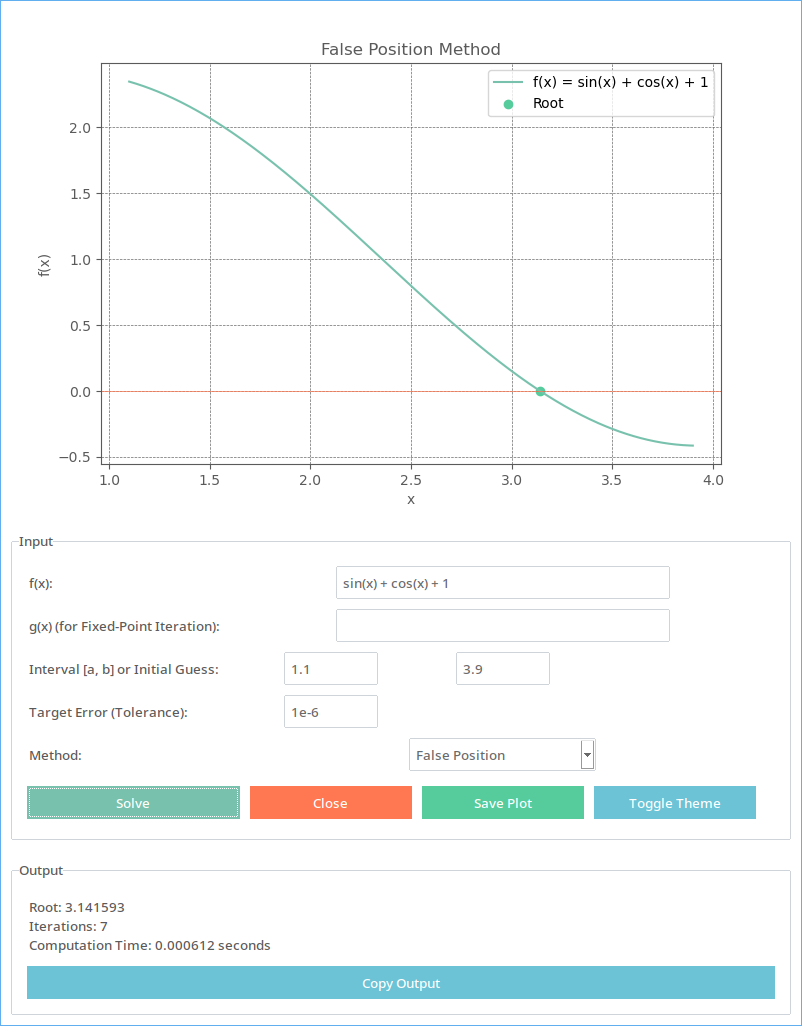
\includegraphics[height=0.5\textwidth]{./fig/ponto-falso.png}
	\caption{Gráfico da falsa posição $[1.1, 3.9]$.}
	\label{fig:grafico-fp}
\end{figure}

\subsubsection{\textbf{Método do Ponto Fixo}}

Aplicando o método do ponto fixo com a função \\ $g(x) = x - 0.5 ⋅ (sin(x) +
	cos(x) + 1)$ e uma estimativa inicial de 1.1, o método convergiu para a raiz
−1,570796 em 20 iterações. O gráfico abaixo ilustra a convergência:

\begin{figure}[H]
	\centering
	\setlength{\fboxsep}{0pt}
	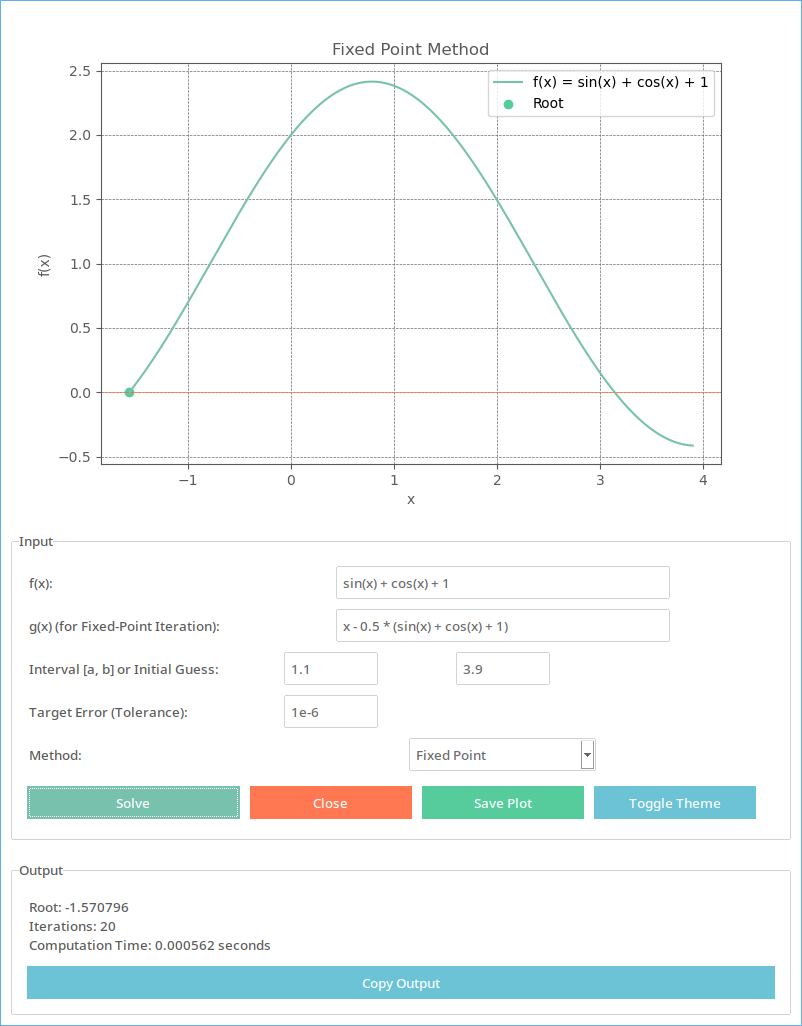
\includegraphics[height=0.5\textwidth]{./fig/ponto-fixo.png}
	\caption{Gráfico do ponto fixo $[1.1, 3.9]$.}
	\label{fig:grafico-pf}
\end{figure}

\subsubsection{\textbf{Método da Secante}}
Por fim, utilizando o método da secante com as estimativas iniciais 1.1 e 3.9,
encontramos a raiz
3,141593 em 6 iterações. O gráfico a seguir mostra a convergência do método:

\begin{figure}[H]
	\centering
	\setlength{\fboxsep}{0pt}
	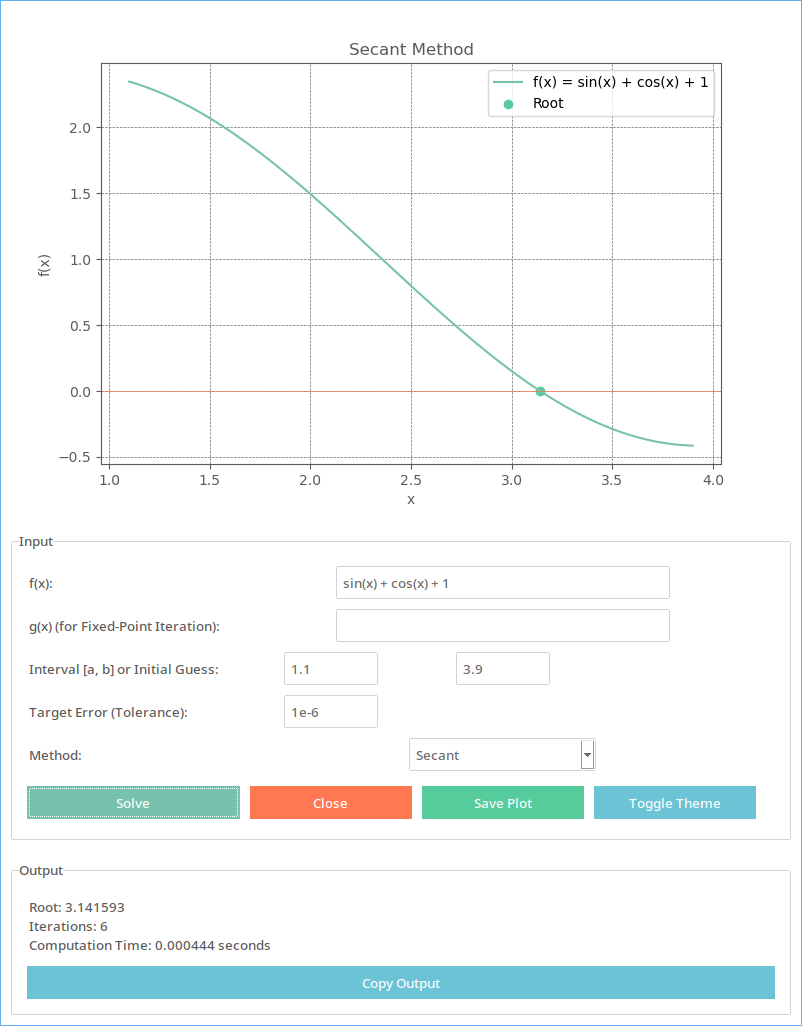
\includegraphics[height=0.5\textwidth]{./fig/secante.png}
	\caption{Gráfico da secante $[1.1, 3.9]$.}
	\label{fig:grafico-sec}
\end{figure}


\begin{figure*}[htbp]
	\centering
	\setlength{\fboxsep}{0pt}
	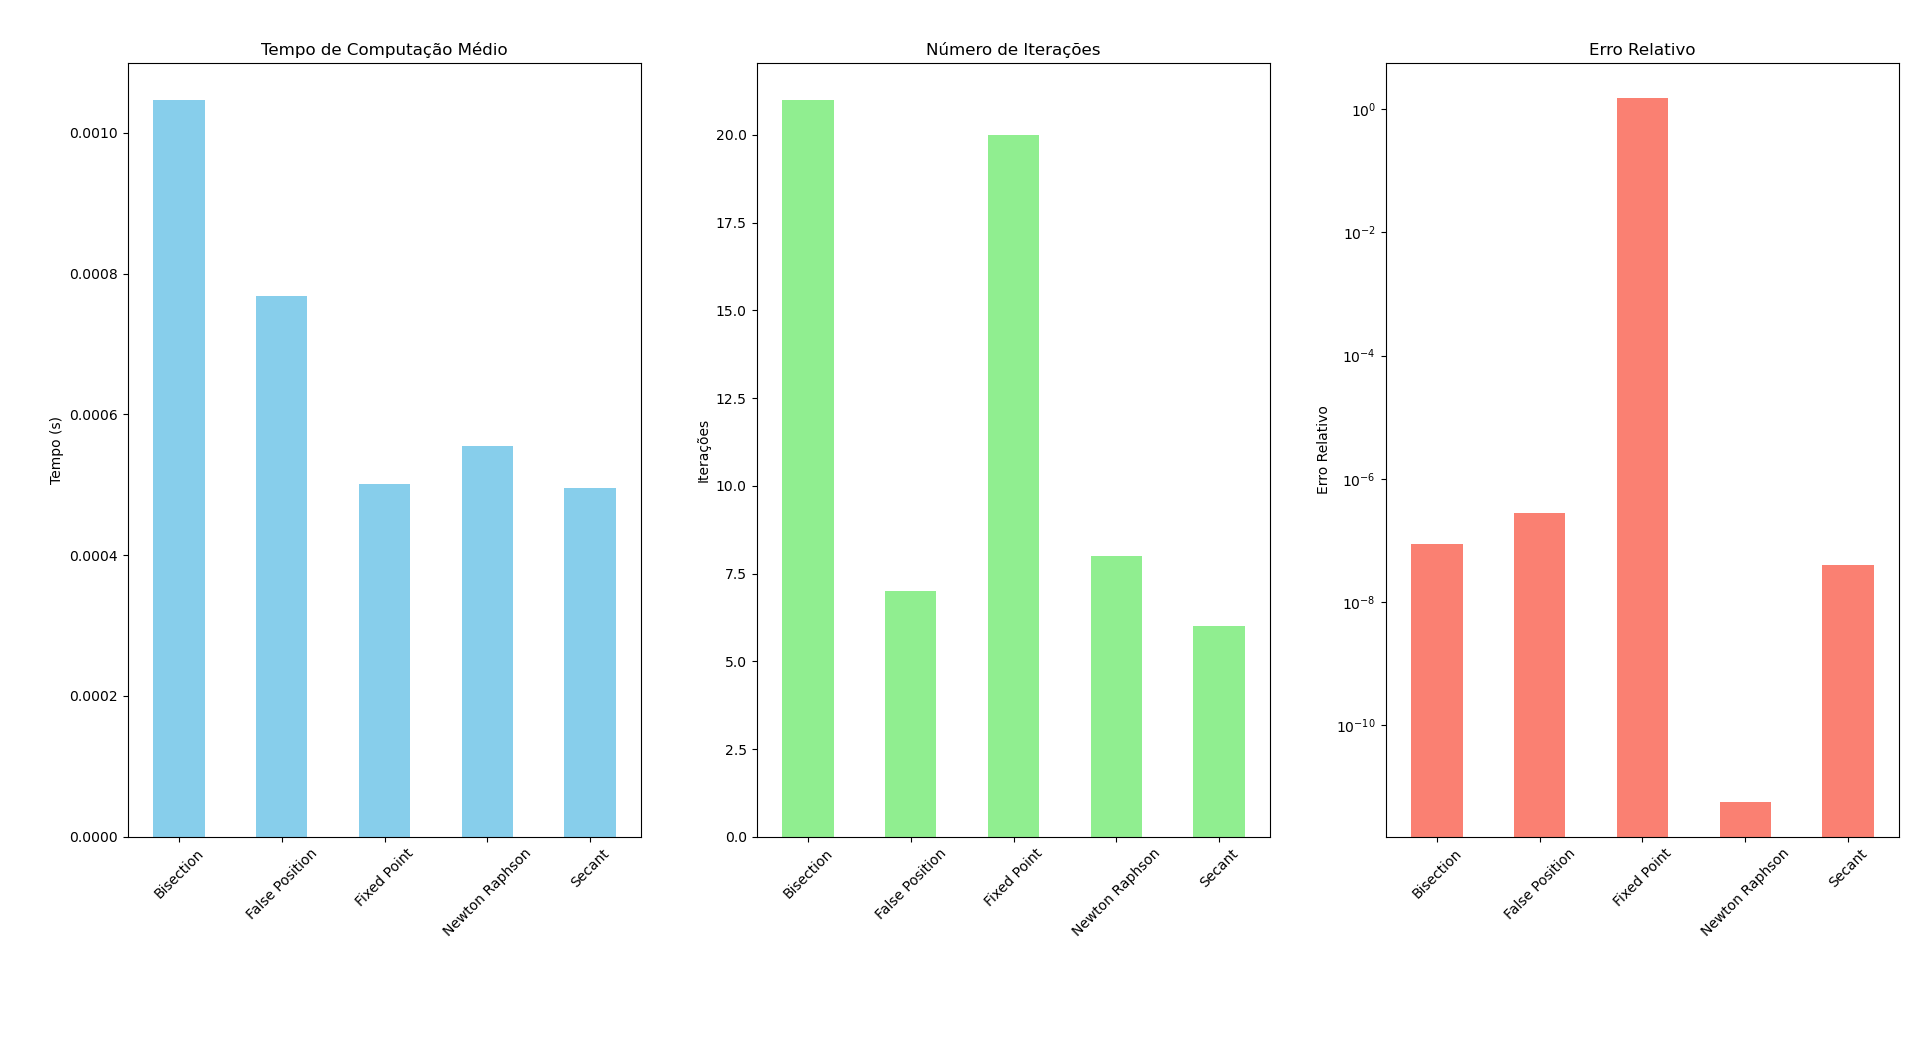
\includegraphics[width=\textwidth]{./fig/benchmark.png}
	\caption{Gráfico comparativo $[1.1, 3.9]$.}
	\label{fig:grafico-comp}
\end{figure*}

\subsection{\textbf{Análise e Comparação}}

Dessa forma, é realizada uma análise comparativa dos métodos numéricos aplicados
à função $f(x) = sin(x) + cos(x) + 1$, considerando o tempo de computação, o
número de iterações e o erro relativo. O gráfico resume os dados
obtidos.\cite{ruggiero1996calculo}~\cite{asano2009calculo}.

Observando de forma geral, é notório como o modo de Newton-Raphson
definitivamente é um dos métodos mais eficientes, devido a seu tempo de execução
satisfatório e baixo erro relativo. Diferentemente do método da bisseção, que
gastou muito tempo de execução e um número muito alto de
iterações.\cite{dequadros2009fundamentos}~\cite{moreira2011curso}.

\subsection{\textbf{Limitações}}

Embora os métodos numéricos sejam ferramentas poderosas para encontrar raízes de
funções, cada um deles possui limitações que devem ser consideradas ao escolher
a abordagem mais adequada para um problema específico. Alguns métodos exigem um
número muito elevado de iterações para atingir a precisão desejada (bisseção),
enquanto outros necessitam de valores iniciais adequados para garantir a
convergência (Newton e secante). Além disso, funções altamente não lineares
podem ser um empecilho para determinados métodos (posição falsa e bisseção), e
uma má escolha da função $g(x)$ pode ser um grande problema para o método do
ponto fixo.\cite{marins1996localizacao}~\cite{lobao_introducao}.

Assim, a junção de todas essas limitações acaba restringindo o desempenho do
software, especialmente quando utilizado por alguém que não domina os
conhecimentos necessários de cálculo numérico, o que pode resultar em resultados
imprecisos.\cite{anton2014calculo}~\cite{bartle1983elementos}.
